\chapter{Arhitektura i dizajn sustava}

		Arhitektura se može podijeliti na tri podsustava:
		\begin{itemize}
			\item 	Web poslužitelj
			\item 	Web aplikacija
			\item 	Baza podataka		
		\end{itemize}

		\underbar{Web preglednik} predstavlja softverski program koji omogućuje korisnicima 
		pregledavanje web-stranica i konzumiranje povezanih multimedijskih sadržaja. 
		Svaki internetski preglednik djeluje kao prevoditelj, interpretirajući kôd web 
		stranica napisan u određenom programskom jeziku i pretvarajući ga u vizualni 
		format razumljiv svakom korisniku. Drugim riječima, stranice su izvorno napisane 
		u kodu, a \textit{web preglednik} ih interpretira kako bi korisnicima pružio čitljiv i 
		interaktivan prikaz. Kada korisnik želi pristupiti određenoj web stranici, 
		šalje zahtjev \textit{web poslužitelju} putem \textit{web preglednika}, što pokreće proces 
		prijenosa informacija i omogućava korisnicima interakciju s odabranim sadržajem.


		\underbar{Web poslužitelj} temelj je rada web aplikacije. Zadužen je za komunikaciju
		klijenta sa aplikacijom. Međusobna komunikacija odvija se putem HTTP (engl. \textit{Hyper
		Text Transfer Protocol}) protokola, koji je jedan od protokola za prijenos informacija
		na webu.

		Korisnik koristi \textit{web aplikaciju} za obrađivanje željenih zahtjeva.
		\textit{Web aplikacija} gleda zahtjev te ovisno o njemu, pristupa bazi podataka nakon čega
		preko \textit{web poslužitelja} vraća korisniku odgovor u HTML dokumentu koji je 
		vidljiv u \textit{web pregledniku}.

		Programski jezik koji smo odabrali za izradu naše \textit{web aplikacije} je Java, zajedno
		sa Spring Boot radnim okvirom te programski jezik JavaScript zajedno sa React radnim okvirom.

		Ovisno o ulogama u timu, odabrana razvoja okruženja su:

		\begin{itemize}
			\item Frontend - Visual Studio Code
			\item Backend - Intellij IDEA
			\item Dokumentacija - Visual Studio Code		
		\end{itemize}

		Arhitekura sustava zasnivat će se na MVC (Model-View-Controller) konceptu.
		Spring Boot nudi veliku podršku za rad sa Spring MVC-om te kao takav
		odgovara našim zahtjevima (također olakšava konfiguraciju potrebnu za validan rad
		Spring MVC-a).

		MVC koncept omogućava nezavisan razvoj pojedinih dijelova aplikacije te kao takav
		olakšava ispitivanje, razvijanje i dodavanje novih svojstva u aplikaciju.

		\medbreak

		Temeljne komponente MVC koncepta su:
		\begin{itemize}
			\item Model - dinamičke strukture podataka, npr. entitet User, Ingredient...
			\item View - ono što korisnik vidi, vizualizacija podataka
			\item Controller - poveznica između Model-a i View-a, bavi se HTTP zahtjevima i odgovorima		
		\end{itemize}

		\eject
				
		\section{Baza podataka}
			
			\subsection{Opis tablica}
				
				
				\begin{longtblr}[
					label=none,
					entry=none
					]{
						width = \textwidth,
						colspec={|X[6,l]|X[6, l]|X[20, l]|}, 
						rowhead = 1,
					} %definicija širine tablice, širine stupaca, poravnanje i broja redaka naslova tablice
					\hline \SetCell[c=3]{c}{\textbf{users}}	 \\ \hline[3pt]
					\SetCell{LightGreen}id & INT	&  	jedinstveni identifikator korisnika  	\\ \hline
					firstName	& VARCHAR &   ime korisnika	\\ \hline 
					lastName & VARCHAR & prezime korisnika  \\ \hline 
					username & VARCHAR	&  korisničko ime korisnika		\\ \hline
					email & VARCHAR	&  adresa elektroničke pošte korisnika		\\ \hline
					password & VARCHAR	&  hash lozinke		\\ \hline 
					\SetCell{LightBlue} roleId	& VARCHAR &  identifikator razine pristupa korisnika (role.id) 	\\ \hline 
				\end{longtblr}

				\begin{longtblr}[
					label=none,
					entry=none
					]{
						width = \textwidth,
						colspec={|X[6,l]|X[6, l]|X[20, l]|}, 
						rowhead = 1,
					} %definicija širine tablice, širine stupaca, poravnanje i broja redaka naslova tablice
					\hline \SetCell[c=3]{c}{\textbf{userFollow}}	 \\ \hline[3pt]
					\SetCell{LightGreen}id & INT	&  	jedinstveni identifikator praćenja	\\ \hline
					\SetCell{LightBlue} followerId	& INT &   id korisnika koji prati 	(user.id)\\ \hline 
					\SetCell{LightBlue} authorId & INT & id autora kojeg se prati  (user.id)\\ \hline 
					followedAt & TIMESTAMP	&  vrijeme početka praćenja		\\ \hline
				\end{longtblr}
				
				\begin{longtblr}[
					label=none,
					entry=none
					]{
						width = \textwidth,
						colspec={|X[6,l]|X[6, l]|X[20, l]|}, 
						rowhead = 1,
					} %definicija širine tablice, širine stupaca, poravnanje i broja redaka naslova tablice
					\hline \SetCell[c=3]{c}{\textbf{chatMessage}}	 \\ \hline[3pt]
					\SetCell{LightGreen}id & INT	&  	jedinstveni identifikator poruke (user.id)	\\ \hline
					\SetCell{LightBlue} senderId	& INT &  id pošiljatelja (user.id)  	\\ \hline 
					\SetCell{LightBlue} receiverId & INT & id primatelja (user.id) \\ \hline 
					content & VARCHAR	&  sadržaj poruke		\\ \hline
				\end{longtblr}

				\begin{longtblr}[
					label=none,
					entry=none
					]{
						width = \textwidth,
						colspec={|X[6,l]|X[6, l]|X[20, l]|}, 
						rowhead = 1,
					} %definicija širine tablice, širine stupaca, poravnanje i broja redaka naslova tablice
					\hline \SetCell[c=3]{c}{\textbf{communicationTime}}	 \\ \hline[3pt]
					\SetCell{LightGreen}id & INT	&  	jedinstveni identifikator komunikacije 	\\ \hline
					\SetCell{LightGreen}userId	& INT &   jedinstveni identifikator korisnika (user.id)\\ \hline 
					\SetCell{LightGreen}start & TIMESTAMP & početak komunikacije  \\ \hline 
					\SetCell{LightGreen}end & TIMESTAMP	&  kraj komunikacije		\\ \hline
				\end{longtblr}

				\begin{longtblr}[
					label=none,
					entry=none
					]{
						width = \textwidth,
						colspec={|X[6,l]|X[6, l]|X[20, l]|}, 
						rowhead = 1,
					} %definicija širine tablice, širine stupaca, poravnanje i broja redaka naslova tablice
					\hline \SetCell[c=3]{c}{\textbf{recipe}}	 \\ \hline[3pt]
					\SetCell{LightGreen}id & INT	&  	jedinstveni identifikator recepta  	\\ \hline
					\SetCell{LightBlue} ingredientId	& INT &   id sastojka 	(ingredient.id)\\ \hline 
					\SetCell{LightBlue} tagId	& INT &   id oznake	(tag.id)\\ \hline 
					\SetCell{LightBlue} categoryId	& INT &   id kategorije	(category.id)\\ \hline 
					\SetCell{LightBlue} cuisineId & INT & id zemlje podrijetla (cuisine.id) \\ \hline 
					\SetCell{LightBlue} mediaId & INT & id multimedijske stavke (media.id) \\ \hline 
					\SetCell{LightBlue} userId & INT	&  id autora (user.id)	\\ \hline
					title & VARCHAR	&  naslov recepta		\\ \hline
					description & VARCHAR	& opis recepta		\\ \hline 
					cookingTime	& INTERVAL &  vrijeme kuhanja 	\\ \hline 
				\end{longtblr}

				\begin{longtblr}[
					label=none,
					entry=none
					]{
						width = \textwidth,
						colspec={|X[6,l]|X[6, l]|X[20, l]|}, 
						rowhead = 1,
					} %definicija širine tablice, širine stupaca, poravnanje i broja redaka naslova tablice
					\hline \SetCell[c=3]{c}{\textbf{recipeRating}}	 \\ \hline[3pt]
					\SetCell{LightGreen}id & INT	&  	jedinstveni identifikator ocjene  	\\ \hline
					\SetCell{LightBlue} userId & INT	&  id klijenta koji je dao ocjenu (user.id)	\\ \hline 
					\SetCell{LightBlue} recipeId & INT & id recepta (recipe.id) \\ \hline 
					rating& INT	&  ocjena	\\ \hline
					comment & VARCHAR	&  komentar		\\ \hline
					createdAt & TIMESTAMP	& vrijeme nastanka ocjene		\\ \hline  
				\end{longtblr}

				\begin{longtblr}[
					label=none,
					entry=none
					]{
						width = \textwidth,
						colspec={|X[6,l]|X[6, l]|X[20, l]|}, 
						rowhead = 1,
					} %definicija širine tablice, širine stupaca, poravnanje i broja redaka naslova tablice
					\hline \SetCell[c=3]{c}{\textbf{bookmarkedRecipe}}	 \\ \hline[3pt]
					\SetCell{LightGreen}id & INT	&  	jedinstveni identifikator zabilježbe recepta  	\\ \hline
					\SetCell{LightBlue} userId & INT	&  id klijenta koji je dao ocjenu (user.id)	\\ \hline 
					\SetCell{LightBlue} recipeId & INT & id recepta (recipe.id) \\ \hline 
					createdAt & TIMESTAMP	& vrijeme nastanka ocjene		\\ \hline  
				\end{longtblr}

				\begin{longtblr}[
					label=none,
					entry=none
					]{
						width = \textwidth,
						colspec={|X[6,l]|X[6, l]|X[20, l]|}, 
						rowhead = 1,
					} %definicija širine tablice, širine stupaca, poravnanje i broja redaka naslova tablice
					\hline \SetCell[c=3]{c}{\textbf{role}}	 \\ \hline[3pt]
					\SetCell{LightGreen}id & INT	&  	jedinstveni identifikator razine pristupa\\ \hline
					name	& VARCHAR &  ime razine pristupa  	\\ \hline 
				\end{longtblr}

				\begin{longtblr}[
					label=none,
					entry=none
					]{
						width = \textwidth,
						colspec={|X[6,l]|X[6, l]|X[20, l]|}, 
						rowhead = 1,
					} %definicija širine tablice, širine stupaca, poravnanje i broja redaka naslova tablice
					\hline \SetCell[c=3]{c}{\textbf{category}}	 \\ \hline[3pt]
					\SetCell{LightGreen}id & INT	&  	jedinstveni identifikator kategorije\\ \hline
					name	& VARCHAR &  ime kategorije  	\\ \hline 
				\end{longtblr}

				
				\begin{longtblr}[
					label=none,
					entry=none
					]{
						width = \textwidth,
						colspec={|X[6,l]|X[6, l]|X[20, l]|}, 
						rowhead = 1,
					} %definicija širine tablice, širine stupaca, poravnanje i broja redaka naslova tablice
					\hline \SetCell[c=3]{c}{\textbf{tag}}	 \\ \hline[3pt]
					\SetCell{LightGreen}id & INT	&  	jedinstveni identifikator oznake recepta\\ \hline
					name	& VARCHAR &  opis oznake recepta  	\\ \hline 
				\end{longtblr}

				\begin{longtblr}[
					label=none,
					entry=none
					]{
						width = \textwidth,
						colspec={|X[6,l]|X[6, l]|X[20, l]|}, 
						rowhead = 1,
					} %definicija širine tablice, širine stupaca, poravnanje i broja redaka naslova tablice
					\hline \SetCell[c=3]{c}{\textbf{ingredient}}	 \\ \hline[3pt]
					\SetCell{LightGreen}id & INT	&  	jedinstveni identifikator sastojka\\ \hline
					name	& VARCHAR &  ime sastojka  	\\ \hline 
				\end{longtblr}


				\begin{longtblr}[
					label=none,
					entry=none
					]{
						width = \textwidth,
						colspec={|X[6,l]|X[6, l]|X[20, l]|}, 
						rowhead = 1,
					} %definicija širine tablice, širine stupaca, poravnanje i broja redaka naslova tablice
					\hline \SetCell[c=3]{c}{\textbf{cuisine}}	 \\ \hline[3pt]
					\SetCell{LightGreen}id & INT	&  	jedinstveni identifikator zemlje kuhanja\\ \hline
					name	& VARCHAR &  ime zemlje kuhanja  	\\ \hline 
				\end{longtblr}

				\begin{longtblr}[
					label=none,
					entry=none
					]{
						width = \textwidth,
						colspec={|X[6,l]|X[6, l]|X[20, l]|}, 
						rowhead = 1,
					} %definicija širine tablice, širine stupaca, poravnanje i broja redaka naslova tablice
					\hline \SetCell[c=3]{c}{\textbf{video}}	 \\ \hline[3pt]
					\SetCell{LightGreen}id & INT	&  	jedinstveni identifikator videa\\ \hline
					duration	& INTERVAL &  trajanje videa  	\\ \hline 
				\end{longtblr}

				\begin{longtblr}[
					label=none,
					entry=none
					]{
						width = \textwidth,
						colspec={|X[6,l]|X[6, l]|X[20, l]|}, 
						rowhead = 1,
					} %definicija širine tablice, širine stupaca, poravnanje i broja redaka naslova tablice
					\hline \SetCell[c=3]{c}{\textbf{image}}	 \\ \hline[3pt]
					\SetCell{LightGreen}id & INT	&  	jedinstveni identifikator fotografije\\ \hline
					width	& INT &  širina fotografije (px)  	\\ \hline
					height	& INT &  visina fotografije (px)  	\\ \hline
					format  & VARCHAR & format fotografije \\ \hline
				\end{longtblr}

				\begin{longtblr}[
					label=none,
					entry=none
					]{
						width = \textwidth,
						colspec={|X[6,l]|X[6, l]|X[20, l]|}, 
						rowhead = 1,
					} %definicija širine tablice, širine stupaca, poravnanje i broja redaka naslova tablice
					\hline \SetCell[c=3]{c}{\textbf{media}}	 \\ \hline[3pt]
					\SetCell{LightGreen}id & INT	&  	jedinstveni identifikator multimedijske stavke\\ \hline
					\SetCell{LightBlue}recipeId	& INT &  id recepta (px)  	\\ \hline
					key	& VARCHAR &   	naziv datoteke na oblaku\\ \hline
					description  & VARCHAR & opis multimedijske stavke \\ \hline
					uploadDate  & DATE & datum postavljanje multimedijske stavke \\ \hline

				\end{longtblr}
				
				\eject

				
				
			
			\subsection{Dijagram baze podataka}

			\begin{figure}[H]
				\rotatebox{90}{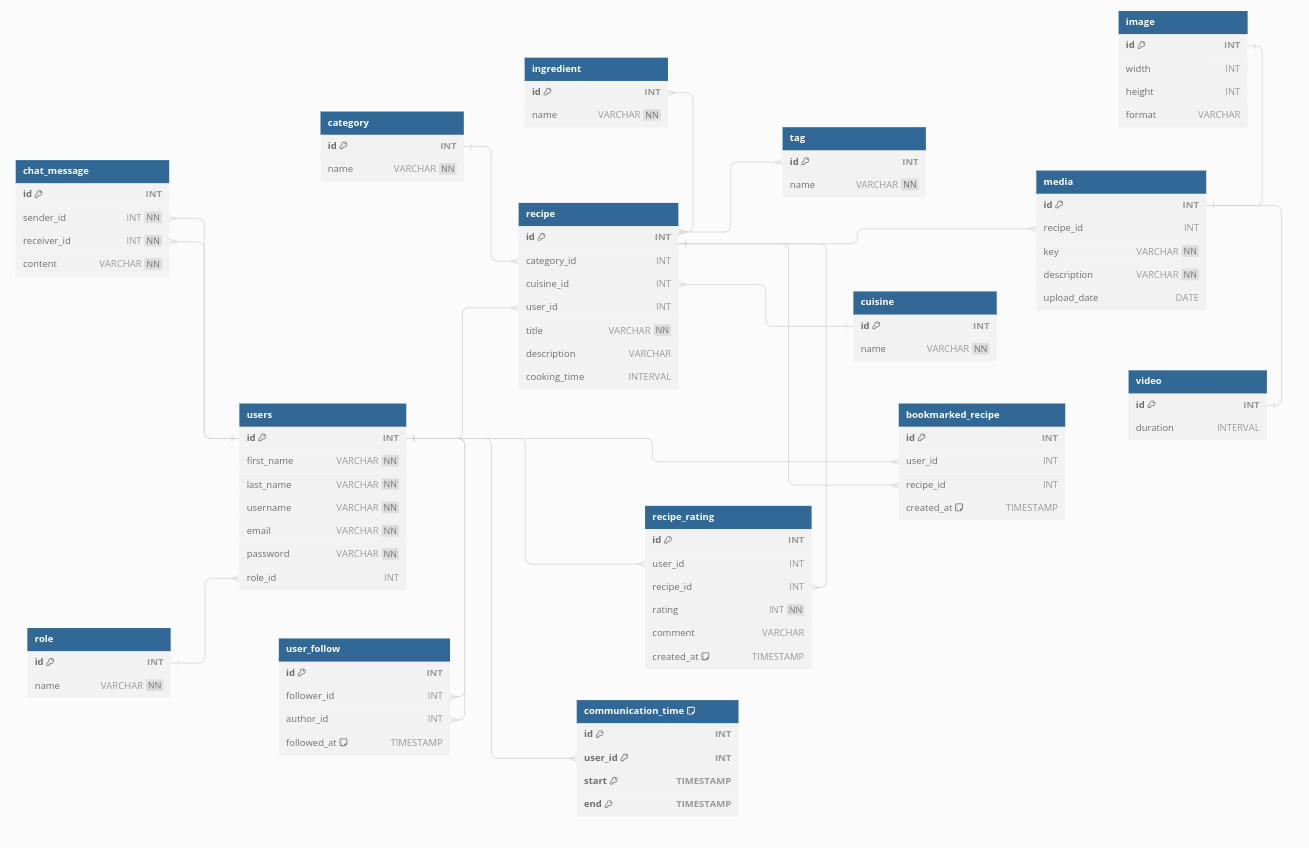
\includegraphics[scale=0.45]{slike/dijagram_baze.png}} 
				\centering
				\caption{Dijagram baze podataka}
				\label{fig:bpdiag}
			\end{figure}
			
			
			\eject
			
			
		\section{Dijagram razreda}
		
			\textit{Potrebno je priložiti dijagram razreda s pripadajućim opisom. Zbog preglednosti je moguće dijagram razlomiti na više njih, ali moraju biti grupirani prema sličnim razinama apstrakcije i srodnim funkcionalnostima.}\\
			
			\textbf{\textit{dio 1. revizije}}\\
			
			\textit{Prilikom prve predaje projekta, potrebno je priložiti potpuno razrađen dijagram razreda vezan uz \textbf{generičku funkcionalnost} sustava. Ostale funkcionalnosti trebaju biti idejno razrađene u dijagramu sa sljedećim komponentama: nazivi razreda, nazivi metoda i vrste pristupa metodama (npr. javni, zaštićeni), nazivi atributa razreda, veze i odnosi između razreda.}\\
			
			\textbf{\textit{dio 2. revizije}}\\			
			
			\textit{Prilikom druge predaje projekta dijagram razreda i opisi moraju odgovarati stvarnom stanju implementacije}
			
			
			
			\eject
		
		\section{Dijagram stanja}
			
			
			\textbf{\textit{dio 2. revizije}}\\
			
			\textit{Potrebno je priložiti dijagram stanja i opisati ga. Dovoljan je jedan dijagram stanja koji prikazuje \textbf{značajan dio funkcionalnosti} sustava. Na primjer, stanja korisničkog sučelja i tijek korištenja neke ključne funkcionalnosti jesu značajan dio sustava, a registracija i prijava nisu. }
			
			
			\eject 
		
		\section{Dijagram aktivnosti}
			
			\textbf{\textit{dio 2. revizije}}\\
			
			 \textit{Potrebno je priložiti dijagram aktivnosti s pripadajućim opisom. Dijagram aktivnosti treba prikazivati značajan dio sustava.}
			
			\eject
		\section{Dijagram komponenti}
		
			\textbf{\textit{dio 2. revizije}}\\
		
			 \textit{Potrebno je priložiti dijagram komponenti s pripadajućim opisom. Dijagram komponenti treba prikazivati strukturu cijele aplikacije.}